Official statistics published by the U.S. government~\cite{EducationPaysBureau} indicate that individuals with doctoral degrees belong to a distinguished group characterized by the highest median weekly earnings and the lowest unemployment rates across the country. With the privilege comes responsibility. In recognizing the advantages my educational status affords me, I am committed to leveraging this privilege to enhance the potential of every student I mentor, particularly within the diverse community at the \appSchool{}.

I acutely recognize that academic diversity encompasses not just identity markers but also varied educational and life backgrounds. My experiences as an international graduate student and a parent during my postdoctoral phase resonate with many students facing similar academic and personal challenges, and I am eager to address the needs of a wider array of students, including transfer students, non-traditional students (e.g., aged 25 and above or those returning to education), student parents, first-generation students, and those academically under-prepared. Capturing this spectrum holistically is essential to crafting a truly inclusive educational environment.


My dedication was reinforced during a routine campus COVID test, where the test administrator was unfamiliar with the term ``postdoc'', revealing a gap in his knowledge of educational pathways, especially regarding doctoral programs and beyond. This interaction continually reminds me of the broader role that an educator can play. As a future faculty member, I am inspired to be a force of enlightenment and change, to open up opportunities to students who may have never known of the intellectual and life options that abound at our university. The influence of these seemingly simple acts of sharing knowledge and creating opportunities is often more profound than it appears.

\begin{figure}[!ht]
    \centering
    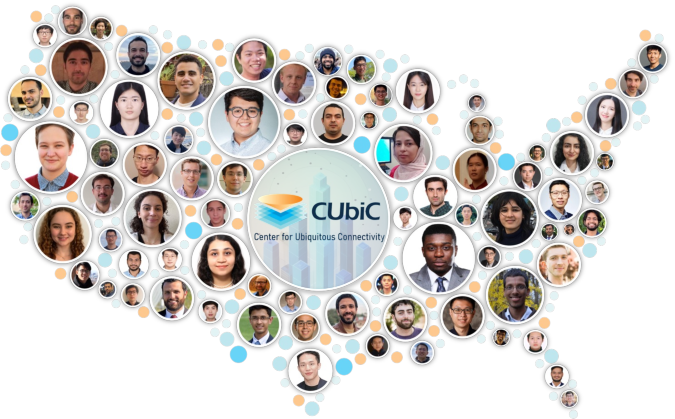
\includegraphics[width=0.5\linewidth]{../../fig/diversity.pdf}
    \caption{Firsthand experience of diversity in action at the SRC JUMP 2.0 Center for Ubiquitous Connectivity (CUbiC) have profoundly shaped my understanding of inclusive mentoring practices.}
    \label{fig:diversity}
\end{figure}

My time at the Center for Ubiquitous Connectivity (CUbiC) under the SRC JUMP 2.0 program has been instrumental in shaping my understanding of practical diversity in action. Diversity is a critical priority in the CUbiC center, as evidenced by the center featuring a female director, a female theme lead, 6 female principal investigators, alongside over 20\% and growing researchers from underrepresented groups. Witnessing the center's inclusive mentoring and outreach programs has demonstrated to me the utmost importance of such initiatives in a research environment. These experiences have provided me with a solid framework for what I aspire to emulate in establishing my own research group in the \appDept{} at the \appSchool{}. In light of these experiences, I formulate my mentoring philosophy guided by a series of introspective questions:

\paragraph{How would I mentor students from diverse backgrounds and with varying research interests or career aspirations?}
My approach is to be student-focused and adaptable. Beyond offering guidance, an essential part of my mentoring role is to listen to and understand the students' unique needs, thereby creating a supportive and collaborative research environment free from distraction. Initially, I will work closely with them to comprehend their interests and provide detailed guidance. As they develop a broader understanding of the field and begin to carve their own research paths, I will encourage independent exploration and collaboration, while always being available for advice and feedback. This approach will evolve with their progress, aligning with their career goals and providing opportunities like internships or teaching roles to build necessary skills.

\paragraph{How would I plan to monitor students' progress?}
Recognizing the variety in learning and research styles, I aim for a balanced approach to meet our common goals such as project deliverables, publications, and pushing the technology forward. I plan to implement a mix of group, project-specific, and individual meetings. Weekly group meetings will facilitate progress sharing and feedback within the group. Project-specific meetings will focus on technical aspects, ensuring detailed progress in a smaller group. One-on-one meetings, which I suggest be bi-weekly but encourage students to proactively reach out, can be leveraged to address a range of topics, from research progress to career advice, depending on the student's pace and needs. In these meetings, I will offer insights from my experience and guide students to appropriate resources.

\paragraph{How would I plan to remain accessible for student inquiries?}
I anticipate managing formal requests and crucial updates predominantly via email, responding promptly or outlining a timeline for detailed follow-up. Moreover, I am adept with alternative communication channels like Slack and aware of the younger generation's preference for more instantaneous platforms like Discord. Considering the post-Covid era where a hybrid of in-person and remote collaboration has become the new norm, I am dedicated to broadening and adapting my availability to enhance communication efficiency.

\paragraph{What expectations do I hold for students approaching graduation?}
My experience with interdisciplinary subjects has made me aware of the varied emphases on publications across different fields, whether it be journal papers or top-tier conferences. While not imposing rigid criteria on publication venues and quantity for students working on diverse topics, a few high-quality, first-author publications with coherent themes are vital for a strong dissertation. Ultimately, I expect a student to confidently claim expertise in their technical area, indicated by their ability to impart new knowledge to me toward the end of their PhD and progressively demonstrate independent research, without the need for an advisor's direction.

\paragraph{How do I ensure sustainable productivity in the long term by encouraging work-life balance?} Acknowledging the intensity and demanding nature of academic pursuits, I prioritize fostering a healthy work-life balance for my students. My approach is to advocate for flexible working hours, understanding that productivity varies across individuals and can often be achieved outside the conventional schedule. Moreover, I emphasize the importance of taking time off, especially following major deadlines or significant project milestones. This approach is intended to prevent burnout and maintain high levels of enthusiasm and creativity in the long term. By recognizing and valuing the need for personal time and recuperation, I aim to cultivate an environment where students feel supported both in their professional growth and personal well-being.\\

My time as a postdoctoral researcher at the Columbia University allowed me to partially implement this philosophy, guiding several Ph.D. students to significant milestones, including publishing their first papers as lead authors at premier conferences and securing their first industry positions. At the \appSchool{}, I look forward to further developing my mentoring philosophy and practices, anchored in recognizing and embracing diversity, fostering an inclusive and supportive academic culture, and encouraging a healthy research environment. I am committed to adapting my approach to meet the unique needs and aspirations of each student, facilitating their journey towards becoming independent and confident scholars. My ultimate goal is to equip the next generation of researchers and innovators with the skills, knowledge, and resilience they need to thrive in their future endeavors, making the pathways to success accessible to all.







